\documentclass[aspectratio=169,12pt]{beamer}
\usepackage{amsmath}
\usepackage{amssymb}
\usepackage[most]{tcolorbox}
\usepackage{tikz}
\usepackage{graphicx}
\usepackage[sfdefault,lf]{FiraSans}
\renewcommand{\familydefault}{\sfdefault}
\setlength{\parindent}{0pt}
\everymath{\displaystyle}

\setbeamertemplate{navigation symbols}{}
\setbeamertemplate{footline}{}
\setbeamertemplate{headline}{}

\definecolor{mmpageWhite}{HTML}{FCFBF7}
\definecolor{mmtanSoft}{HTML}{F7F5EF}
\definecolor{mmgreenDeep}{HTML}{244B2C}
\definecolor{mmgreenLeaf}{HTML}{5D8A56}
\definecolor{mmgreenSoft}{HTML}{E4EFD9}
\definecolor{mmtext}{HTML}{163221}

\setbeamercolor{background canvas}{bg=mmpageWhite}
\setbeamercolor{normal text}{fg=mmtext,bg=mmpageWhite}

\newtcolorbox{MMProblemCard}[1][]{enhanced,breakable=false,colback=white,colframe=black,boxrule=1.0pt,arc=5pt,left=3pt,right=3pt,top=2pt,bottom=2pt,before skip=0pt,after skip=0pt,height=0.26\textheight,valign=top,#1}
\newcommand{\KoruIcon}{\raisebox{-0.2em}{
\includegraphics[height=1.05em]{../../SITE/header-logo.png}}}
\newcommand{\HoeIcon}{\raisebox{-0.2em}{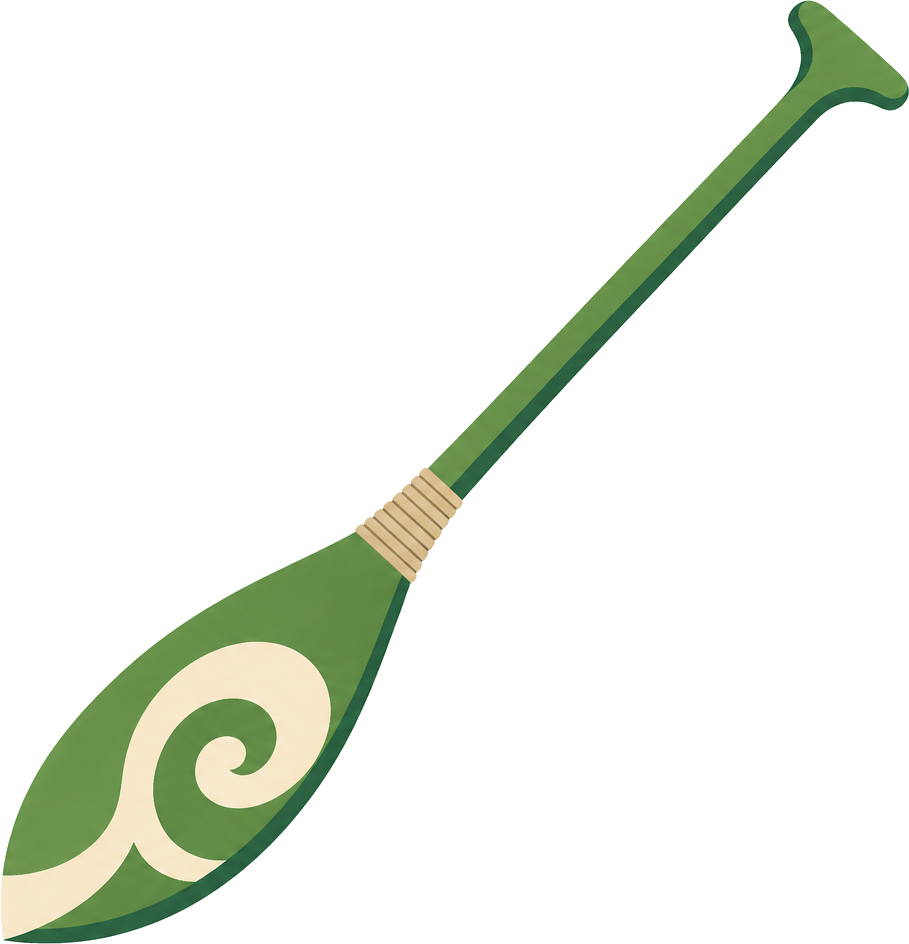
\includegraphics[height=1.05em]{../../SITE/hoe.png}}}
\newcommand{\ScaffoldIcons}[1]{\ifcase#1\or \HoeIcon\or \HoeIcon\hspace{0.22em}\HoeIcon\or \HoeIcon\hspace{0.22em}\HoeIcon\hspace{0.22em}\HoeIcon\fi}
\newcommand{\WorksheetTitle}[2]{%
  {\colorbox{mmtanSoft}{\parbox[c][2.0em][c]{0.975\linewidth}{%
    \hspace{0.25em}{\Large\bfseries\textcolor{mmgreenDeep}{#1}\hfill\ScaffoldIcons{#2}}}}
  \par\vspace{0.08em}{\color{mmgreenLeaf}\rule{\linewidth}{2.0pt}}\par\vspace{0.04em}}
}
\newcommand{\MMProblem}[2]{\begin{MMProblemCard}\raggedright\small\textbf{#1.} #2\par\end{MMProblemCard}}

\setbeamertemplate{background}{
 \begin{tikzpicture}[remember picture,overlay]
 \draw[black,line width=1.5pt,rounded corners=10pt]
 ([xshift=0.45cm,yshift=-0.45cm]current page.north west)
 rectangle
 ([xshift=-0.45cm,yshift=0.45cm]current page.south east);
 \end{tikzpicture}
}

\begin{document}
\begin{frame}[t]
\WorksheetTitle{Push Tasks}{3}
\vspace{-0.18em}
\begin{columns}[T,onlytextwidth]
\begin{column}{0.32\textwidth}\MMProblem{1}{A scale from 0 to 148 has marks every 14. The needle is at 28. Between which two marks is it?}\end{column}
\begin{column}{0.32\textwidth}\MMProblem{2}{A scale from 0 to 73 has marks every 7. The needle is at 28. Between which two marks is it?}\end{column}
\begin{column}{0.32\textwidth}\MMProblem{3}{A scale from 0 to 445 has marks every 63. The needle is at 126. Between which two marks is it?}\end{column}
\end{columns}
\vspace{0.45em}
\begin{columns}[T,onlytextwidth]
\begin{column}{0.32\textwidth}\MMProblem{4}{A scale from 0 to 487 has marks every 81. The needle is at 162. Between which two marks is it?}\end{column}
\begin{column}{0.32\textwidth}\MMProblem{5}{A scale from 0 to 244 has marks every 34. The needle is at 272. Between which two marks is it?}\end{column}
\begin{column}{0.32\textwidth}\MMProblem{6}{A scale from 0 to 375 has marks every 53. The needle is at 159. Between which two marks is it?}\end{column}
\end{columns}
\vspace{0.45em}
\begin{columns}[T,onlytextwidth]
\begin{column}{0.32\textwidth}\MMProblem{7}{A scale from 0 to 239 has marks every 34. The needle is at 136. Between which two marks is it?}\end{column}
\begin{column}{0.32\textwidth}\MMProblem{8}{A scale from 0 to 393 has marks every 56. The needle is at 112. Between which two marks is it?}\end{column}
\begin{column}{0.32\textwidth}\MMProblem{9}{A scale from 0 to 361 has marks every 36. The needle is at 108. Between which two marks is it?}\end{column}
\end{columns}
\end{frame}

\begin{frame}[t]
\WorksheetTitle{Push Tasks}{3}
\vspace{-0.18em}
\begin{columns}[T,onlytextwidth]
\begin{column}{0.32\textwidth}\MMProblem{10}{A scale from 0 to 323 has marks every 32. The needle is at 128. Between which two marks is it?}\end{column}
\begin{column}{0.32\textwidth}\MMProblem{11}{A scale from 0 to 133 has marks every 16. The needle is at 112. Between which two marks is it?}\end{column}
\begin{column}{0.32\textwidth}\MMProblem{12}{A scale from 0 to 188 has marks every 18. The needle is at 72. Between which two marks is it?}\end{column}
\end{columns}
\vspace{0.45em}
\begin{columns}[T,onlytextwidth]
\begin{column}{0.32\textwidth}\MMProblem{13}{A scale from 0 to 400 has marks every 57. The needle is at 57. Between which two marks is it?}\end{column}
\begin{column}{0.32\textwidth}\MMProblem{14}{A scale from 0 to 167 has marks every 33. The needle is at 198. Between which two marks is it?}\end{column}
\begin{column}{0.32\textwidth}\MMProblem{15}{A scale from 0 to 255 has marks every 36. The needle is at 72. Between which two marks is it?}\end{column}
\end{columns}
\vspace{0.45em}
\begin{columns}[T,onlytextwidth]
\begin{column}{0.32\textwidth}\MMProblem{16}{A scale from 0 to 158 has marks every 17. The needle is at 102. Between which two marks is it?}\end{column}
\begin{column}{0.32\textwidth}\MMProblem{17}{A scale from 0 to 158 has marks every 15. The needle is at 120. Between which two marks is it?}\end{column}
\begin{column}{0.32\textwidth}\MMProblem{18}{A scale from 0 to 252 has marks every 25. The needle is at 200. Between which two marks is it?}\end{column}
\end{columns}
\end{frame}

\begin{frame}[t]
\WorksheetTitle{Push Tasks}{3}
\vspace{-0.18em}
\begin{columns}[T,onlytextwidth]
\begin{column}{0.32\textwidth}\MMProblem{19}{A scale from 0 to 123 has marks every 17. The needle is at 51. Between which two marks is it?}\end{column}
\begin{column}{0.32\textwidth}\MMProblem{20}{A scale from 0 to 176 has marks every 17. The needle is at 85. Between which two marks is it?}\end{column}
\begin{column}{0.32\textwidth}\MMProblem{21}{A scale from 0 to 432 has marks every 48. The needle is at 336. Between which two marks is it?}\end{column}
\end{columns}
\vspace{0.45em}
\begin{columns}[T,onlytextwidth]
\begin{column}{0.32\textwidth}\MMProblem{22}{A scale from 0 to 348 has marks every 43. The needle is at 258. Between which two marks is it?}\end{column}
\begin{column}{0.32\textwidth}\MMProblem{23}{A scale from 0 to 162 has marks every 27. The needle is at 216. Between which two marks is it?}\end{column}
\begin{column}{0.32\textwidth}\MMProblem{24}{A scale from 0 to 96 has marks every 19. The needle is at 38. Between which two marks is it?}\end{column}
\end{columns}
\vspace{0.45em}
\begin{columns}[T,onlytextwidth]
\begin{column}{0.32\textwidth}\MMProblem{25}{A scale from 0 to 128 has marks every 12. The needle is at 36. Between which two marks is it?}\end{column}
\begin{column}{0.32\textwidth}\MMProblem{26}{A scale from 0 to 455 has marks every 45. The needle is at 315. Between which two marks is it?}\end{column}
\begin{column}{0.32\textwidth}\MMProblem{27}{A scale from 0 to 355 has marks every 71. The needle is at 497. Between which two marks is it?}\end{column}
\end{columns}
\end{frame}
\end{document}
